%------------------------------------------------------------------------------------
% Template for graduated students 2019 - 2020 Research Project
%
% The fonts, linespacing, numbering, page styles, order
% of  Title/Abstract/TOC/Body/{Appendices}/Acknowledgements/References 
% are prescribed as the FMS house style.
%
% Do not change them or add to it without getting approval first.
% Dissertations are not accepted if they do not follow house style.
%------------------------------------------------------------------------------------
\documentclass{fms}
\usepackage[utf8]{inputenc}
\usepackage[numbers]{natbib}
\usepackage[english]{babel}
\usepackage{algorithm}
%------------------------------------------------------------------------------------
% To use external packages for specific needs, uncomment the correct line
% or add your own line (they should not override general FMS house style and layout).
%
\usepackage[pdftex]{graphicx}

%% Load caption before arabtex
%\usepackage{caption} %many figures in one figure (subfigure and subfig are deprecated) 
%\usepackage{subcaption} %many figures in one figure (subfigure and subfig are deprecated)

%% For tables:
%\usepackage{etex}
%\usepackage{booktabs} % \toprule, \midrule, \bottomrule
%\usepackage{array}    % \newcolumntype
%\usepackage{multirow}
%\usepackage{color, colortbl}
%\definecolor{Gray}{gray}{0.8}
%\definecolor{LightCyan}{rgb}{0.88,1,1}
%\usepackage{arydshln}

%% For figures:
%\usepackage[below,section]{placeins} % use \FloatBarrier in the body to really force
% a float somewhere. Please limit use.
%% \usepackage{float}  %"H" placement spec, for **really here** (i.e. not float)
%
%% For code and algorithms
%\usepackage{moreverb}   % \verbatimtabinput
%% \usepackage{listings} % more flexible and complicated 
%                        % than moreverb and algorithm
%% For links and hyper references
%\urlstyle{same}

%% others
%\usepackage{parskip}
\usepackage{enumerate}
%\usepackage{tikz}
%\usepackage{rotating}
%\usepackage{multicol}
\usepackage{algorithm,algorithmic}
%\usepackage{bbm}
\usepackage{epsfig}
\usepackage{graphicx}
\usepackage[all]{xy}

% For Theorems and such, use the environments defined here:
% \begin{thm}...\end{thm} (or "lem", "defn", etc)
\newtheorem{defi}{Definition}[chapter]
\renewcommand{\thedefi}{\arabic{chapter}.\arabic{section}.\arabic{defi}}

\newtheorem{theorem}{Theorem}[chapter]
\renewcommand{\thetheorem}{\arabic{chapter}.\arabic{section}.\arabic{theorem}}

\newtheorem{example}{Example}[chapter]
\renewcommand{\theexample}{\arabic{chapter}.\arabic{section}.\arabic{example}}

\newtheorem{lemma}{Lemma}[chapter]
\renewcommand{\thelemma}{\arabic{chapter}.\arabic{section}.\arabic{lemma}}

\newtheorem{pro}{Proposition}[chapter]
\renewcommand{\thepro}{\arabic{chapter}.\arabic{section}.\arabic{pro}}

%---------------------------------------------------------------------------------------
\begin{document}
\begin{titlepage}
\begin{center}
%
{\begin{picture}(0,0)\unitlength=1.0cm
\put(-1.3,-1){

\includegraphics[width=0.15\textwidth]{images/UofK_logo.jpg}
}
\end{picture}
}\\ \vspace{1.5cm} 
{\large Department of Applied Mathematics \par} \vspace{0.05cm}
{\large Faculty of Mathematical Sciences \par} \vspace{0.05cm}
{\large University of Khartoum \par} \vspace{2.5cm}
{\Huge \textbf{Group Testing Via Binary Matrices} \par} \vspace{2cm}
{\large A dissertation submitted to the Faculty of Mathematical Sciences, University of Khartoum in partial fulfillment of the requirements for the degree of Msc in pure mathematics (Mathematics) \par} \vspace{1.0cm} 

\

\




{\large By:
\large \textbf{Khalid Omer Elamin Hassan}   
\par} \vspace{1.25cm}
{\large Supervisor: \par} 
{\large Dr. AbdElnasir Degoot \par} \vspace{0.6cm}
\vfill 
{\small July, 2022}
%
\end{center}
\end{titlepage}


\pagestyle{empty}
\pagenumbering{roman}
%--------------------------------------------------------------------------------------
% All other files are input via \include. 
% To compile in texmaker while viewing any of those without having to switch back, use
% Options > Define Current Document as 'Master Document'.
% To not have to close a PDF, remove viewpdf from quickbuild and open the PDF (once)
% manually: it will auto-refresh or with control-r
% --------------------------------------------------------------------------------------
% An FMS Dissertation can use the sectioning commands "\chapter", "\section",
% "\subsection". No "\subsubsection", "\paragraph", etc. They are disabled.
%---------------------------------------------------------------------------------------
% See the acknowledgement.tex file and follow the instructions there.
\chapter*{ACKNOWLEDGEMENTS}
\addcontentsline{toc}{chapter}{Acknowledgements}
% We do not number this or add it to the contents!
% Overly long acknowledgements are not professional.
%
% Note LaTeX Produce an error when \\ is used in normal text 

 I would like to thank Dr. Abdoelnaser Degoot, who has not saved any effort in helping me finishing this work.  His valuable feedbacks and comments were a source of knowledge and encouragement and helped taking the work to another level.  
  
Also, I would like to thank my family and friends for their continuous support and encouragement.
%\newpage

%\chapter*{DEDICATION} 
%\addcontentsline{toc}{chapter}{Dedication}
% Don't change anything above this.
\
\

\
\
\
\

\

%{\large  To my mother..I love you..
\chapter*{Abstract}
\addcontentsline{toc}{chapter}{Abstract}
%
% Note LaTeX Produce an error when \\ is used in normal text 
%
%A short description of your whole dissertation goes here. This should be between 100 and 300 words long. But write it last.

%An abstract is not a summary of your essay: it's an abstraction of that. 
%It tells the readers why they should be interested in your essay but summarises all 
%they need to know if they read no further.

%The writing style used in an abstract is like the style used in the rest of your essay: concise, clear and direct. 
%In the rest of the essay, however, you will introduce and use technical terms. In the abstract you should
%avoid them in order to make the result comprehensible to all.

Rapid detection of individuals infected of viruses like Covid-19 is vital in controlling the spread of the disease. The traditional approach to testing (detection) is a test per individual, which is expensive, time consuming and requires large medical capacities.  

The goal of group testing is minimize the number of tests required to identify an infected individual in a population. A test in the context of group testing is an action on a group of individuals that is positive if at least of one of the tested is infected and negative otherwise. Generally, there are two kinds types of group tests, adaptive tests and non-adaptive test. In this work we consider the non-adaptive tests, where the tests are fixed in advance and conducted in parallel. The modeling problem is centered on retrieving a missing information of infected from the tests designs and the outcome of the tests a process also known as decoding.    


We present two topics here, the construction of efficient test designs. With the perfect design we can reduce the cost decoding, time and storage wise.  The second we review an algorithm that works on retrieving the missing information.  Here we verify that The Hard thresholding algorithms are robust and accurate in the decoding process.  
\tableofcontents
\listoffigures
\addcontentsline{toc}{chapter}{List of Figures}
% 
% Figures may differ between topics, but they are not there to fill the pages - they
% must add meaning. In general most figures should be 0.75 times the width of the page
% (perhaps wider in total when two or three columns of figures)
% See the example in chapter one for defining that. Be *consistent*
% in your presentation of information.
%
%\listoftables
%\addcontentsline{toc}{chapter}{List of Tables}
\newpage
\pagenumbering{arabic}
%-----------------------------------------------------------------------------------------
% content (chapters) go in separate files
\pagestyle{myheadings}
% Note LaTeX Produce an error when \\ is used in normal text 
\chapter{Introduction}
%






\section{General introduction}
Late 2019 marked the beginning of the spread of SARS-Covid19 where it first appeared in Wuhan China and quickly spread to the rest of the world. Because of the infectious nature of the disease its spread was rapid. Many countries suffered from it, the health systems and facilities have been overwhelmed and failed to meet the demand. To control its transmission governments imposed many measures but the rapid detection of the infectious cases is crucial to contain the disease. Therefore, governments and health organizations conducted massive testing on the population. With this comes another problem that is, large scale testing is very expensive and needs big capacity.  

Group  testing or pool testing has been used in many countries. It was first studied by Robert Dorfman in the United states during the second world war, where a large number of new recruits of the army were tested for Syphilis \cite{kubook}.

The samples to be tested are taken from a group (pool) rather than individuals. The population is divided into groups and then a sample representing a mixture of each individual sample in the group is tested. If the test result of a particular mixture is negative then all the individuals in the group are free of the disease. If the test comes out positive, then at least one individual in the group is infected. Several tests of such kind can be used to determine the infected individuals of the population in contrast to the traditional way where each individual is tested alone. With arranging the procedure carefully as precise tests, good selection of groups, this would reduce the number of tests dramatically.       

In general, suppose that we have \textit{n} number of individuals to be tested. The traditional way is to conduct \textit{n} number of tests, that is one test per individual. If the number of infected is large then this would be reasonable. By the time of Dorfman's work, the U.S army was testing the new recruits for Syphilis, and it was rare among the population and he started studying pool testing \cite{aldridge}.

The problem can be described as, given a number of items (persons) n and number of defectives (infected) $d$, then how many tests $t$ are required to discover the number of defected (infected) among the $n$ items (persons) and what is feasible way  to achieve this \cite{aldridge}.  

This problem can be classified depending on the point of view that is taken into consideration.


\section{Mathematical background}
The problem is to reconstruct the missing information (detection) from the measured data. The basic assumption is that the information is obtained and processed following a linear model, that is the problem is reduced to solving a system of linear equations. Suppose that the results from the laboratory are referred to as $ y \in \mathbb{R}^n $,  which corresponds to $ x \in \mathbb{R}^n $. $ x $ represents the information about the detection of the infected. 

The problem is formalized as follows: 
\begin{equation}\label{equation1}
Ax = y 
\end{equation} The matrix $ A \in \mathbb{R}^{m \times n}$ \quad is called the design matrix, which represents the testing process, $ m $ is the number of tests and $ n $ is the number of people tested \cite{mathbook}. 

The aim is to recover the vector $ x \in \mathbb{R}^n $ by solving  Eq.(\ref{equation1}) for $ x $. Ideally, $ m = n $ hence the system is easily solved but it is common to have $ m < n $ since the problem states that. Linear algebra tells us that this system is undetermined and it has infinitely many solutions. This renders the problem impossible to solve, $ i.e. $ recover the exact vector $ x $. However, under certain assumptions it is possible to have a solution of the problem, and there are efficient algorithms to recover $ x $ exactly. The assumption is the referred to as the \textbf{Sparsity}. 

\textbf{Sparsity}: a vector is said to be sparse if most of its components are zeros. Formally, a vector $ x \in \mathbb{R}^n $ \quad is called $ s$-sparse  if at most $ s $ of components are non-zeros.  Linking this to our work is, since the vector $ x $ in eq. \ref{equation1} represents the individuals to be test among which some of them are infected, with knowledge of the infectious rate and it assumed to be small, then with zero represents being free of the disease, then it is appealing to consider that our vector is sparse \cite{mathbook}. 

In general, looking at the problem of reconstructing  $ x $, one would address two main questions \cite{mathbook}: 

\begin{itemize}
	\item What is the best matrix $ A^{m\times n} $   \quad that one uses to obtain the best results? 
	\item What is the efficient algorithm that one uses to reconstruct $ x $ from $ Ax = y $?   
\end{itemize}   
\section{Adaptive and non-adaptive group testing}
\subsection{Adaptive (sequential) tests}
In Adaptive (sequential) algorithms, the tests are conducted sequentially one by one. The results from one test are recorded and used in the next test \cite{kubook}. For instance, imagine a situation of testing 100 individuals for Covid19. At the beginning two groups are formed and one assumes one of the groups is free of the virus. thus for the second round of testing the knowledge from the first test is used as that, all the individuals in the first group are discarded and the second group is divided into smaller distinct groups. 
\subsection{Non-adaptive tests}
In the non-adaptive algorithms, the groups to be tested are determined in advance, the tests are conducted in parallel and an individual can be involved in more than one test. It is intuitive that non-adaptive tests are time saving, and in our case, the covid19, where the tests must be conducted simultaneously, this is advantageous \cite{aldridge}. 

However, in general the adaptive tests are faster than non-adaptive because it transfers information from the previous tests to next tests. Considering the advantages from both types it is appealing to try to treat one test like the other. Non-adaptive tests can be treated as adaptive by staging the tests. Here the tests are divided into stages and information is transferred from one stage to the next, but within the stage information is not shared \cite{kubook}.



Although the two questions raised above are connected since the design matrix is part of the algorithm to be used, it is often helpful to try to answer them separately.   
Next we introduce common terminologies of the groups testing models that determine our definition of the model being successful i.e. achieving the best results with a minimum number of tests.

\begin{enumerate}
	\item Binary and non-binary: In the standard group testing model, the design matrix, the defective vector and the outcomes vector are all in binary form. Where 0 in the design matrix represents not being tested and 1 otherwise, while in the defectives and the outcomes vectors, 0 for being free of the virus and 1 otherwise. Other models consider non-binary representation \cite{aldridge}. In this work we will consider the binary representation. The use of the binary setting is beneficial whereas it allows to use the literature of compressive sensing problem \cite{kubook}.   
	\item Noise: Noiseless are tests where there is no error of any kind, that is the recovery is done complete, i.e. the test procedures are done perfect. While in noisy tests we expect errors to happen either from the model or other reasons for example human errors. Two common model errors  are the false positive (specificity) or false negative (sensitivity), where the former the negative outcome is labeled positive by the algorithm and later a positive outcome is labeled negative. In the realistic models small error probability is allowed, where the set of defective individuals is taken to be the defectives with high probability \cite{kubook}. 
	
	\item In our work here we consider a situation where the number of infected is known in advance through the knowledge of the infectious rate. The problem is combinatorial as the set of defectives (infected) is uniformly random among the sets of its size.    
\end{enumerate}

Our work will focus on the combinatorial non-adaptive tests and its implementation  by building in-silico  simulations of a non-adaptive test. 

\section{Useful terms and definitions}
\begin{enumerate}
	\item \textbf{Defective set}: We refer to the number of elements to be tested as n. We write $ D = \{1,2, ..., n\} $ for the set of defectives where each number item in the list is a label given to each individual  and $ d  = |D|$ is the number of defectives.
	
	We write $ x_i  = 1$ for the defective (infected) item   $i\in D $ and $ x_i = 0 $ for non defective (infected) item $ i \notin D $.
	\item \textbf{Tests}: we refer to the number of tests performed or to be performed by $m$, and label the tests $ \{1,2,3 ..., m\} $. The tests represent the rows of the matrix $ A $ where the element $ a_{ij} $ is element $ j $ of $ n $ and tested in the $ i^{th} $ test. An important consideration is that each item is included in each test independently with fixed probability. The matrices we will use are sparse matrices. Although there is no particular criterion to judge exactly if a matrix is sparse or not it is common to set the number of non zero elements to be equal to the number of rows or columns of the matrix \cite{aldridge}. Note that throughout this text we will refer to this matrix by $ A $ or if else it will be stated.   
	\item \textbf{Standard noiseless group testing model} for known $m,n$ and a test matrix $ A^{m\times n} $ this model is described by its outcomes as follows:
	
	\begin{center} $y_{j} =$  
		$\begin{cases}
		1 & if \quad \exists   i \in D  \quad \text{with}  \quad x_{ij} = 1\\
		0 & if \quad \exists   i \in D  \quad with  \quad x_{ij} = 0
		\end{cases}$
	\end{center}
	where $ y_j $ $ \in \{0,1\}^m $ is the test outcome \cite{aldridge}.
	\item \textbf{Detection algorithm}:
	It is a function (map) that maps an element of the set $ \{0,1\}^{m\times n} \times \{0,1\}^m $ to the subsets of $ \{1,2,..., n\} $. Under an ideal recovery the output of the function above is the set of defectives (infected) \cite{aldridge}.  
%	\item \textbf{Zero and first norms}: The zero norm $ l_0  $,  counts the number of non-zero entries of a sparse vector. While the first norm, $ l_1 $,  is the usual taxi-cab norm defined by the summation of the absolute values of the respected components of the considered vectors.      
  

\item{\textbf{Norms}}

A norm of a vector space is a mapping that associates with each vector $ v $ a real number $||v||$ such that the following properties are satisfied for all vectors $ u, v $ and all scalars $ c \in \mathbb{R} $; 
\begin{enumerate}
	\item $ ||v|| \geq 0 $ and $ ||v|| = 0 $ if and only if $ v = 0 $.
	\item $||cv|| = |c| ||v||$.
	\item $||u+v|| \leq ||u|| + ||v||$
\end{enumerate}
The general norm in $ \mathbb{R} $ is defined as follows: 
\begin{equation}\label{key}
||v||_p = (|v_1|^p + ... + |v_n|^p)^{\frac{1}{p}}
\end{equation}
The first norm $ ||v||_1 $ also known as the taxicab is then obtained by setting $ p = 1 $ \begin{equation}\label{key}
||v||_1 = |v_1| + |v_2| + ... + |v_n|
\end{equation}
The second norm of the usual euclidean norm is obtained by setting $ p = 2 $ \begin{equation}\label{key}
||v||_2 = (|v_1|^2+...+|v_n|^2)^{\frac{1}{2}}
\end{equation} 

While as for the $ ||v||_0 $ or the pseudo norm is actually a comparison tool rather being the literal norm defined above, the $ ||v||_0 $ or $ l_0 $ as refereed to in the text  between counts the number of nonzero components in a vector. 
\item{\textbf{Matrix norms induced by  p-norms}}

A matrix norm on $ M_{nn} : V^{m\times n} \longrightarrow \mathbf{R}$ is a mapping that associates with $ m\times n $ matrix $ A $ a real number $ ||A|| $ called the norm of $ A $, such that the following properties are satisfied for all $ m \times n $ matrices and scalar $ \alpha \in V$ \begin{enumerate}
	\item $ ||A|| \geq 0 $.
	\item $ ||A|| = 0 \Longleftrightarrow A = 0_{m\times n} $. 
	\item $ ||\alpha A|| = |\alpha| ||A||$.
	\item $ ||A+B|| \leq ||A|| + ||B|| $.
\end{enumerate}

For $ 1 \geq p \leq \infty$ the corresponding operator norm is \begin{equation} ||A||_p = sup_{x \neq 0} \frac{||Ax||_p}{||x||_p} \end{equation} 
For the special cases $ p = 1,2$ the matrix norm is defined as follows: \begin{equation}
||A||_1 = max_{1\leq j \leq n} \sum_{i =1}^{m} |a_{ij} |
\end{equation}
\begin{equation}
||A||_2 = \sigma_{max} (A) 
\end{equation} where $\sigma_{max} (A)$ is the square root of the largest eigen value of $ AA^{T} $.
\end{enumerate}    

 % Introduction is usually a chapter itself.
\chapter{The Recovery Process}  
%
In this chapter we describe the path which we took to recover the missing vector of infection and  building the in-silico simulation. First we start by re mentioning the questions that need to be answered to build a good group testing model. First, what is the best matrix that one uses to obtain best results. this question is important as the rows of the matrix represent the number of tests to be ran, so fewer rows are better, but also this should not come at a cost of the recovery. The second question concerns the best algorithm to be used in order to get the best recovery results. Here in this chapter we focus on an iterative algorithms called the Hard thresholding algorithms. %Where we write an implantation of the algorithms using programming language Python as well as running some performance tests.
\section{The measurement matrix}
\label{label1}
Our goal is to solve the minimization problem which is sometimes referred to as the basis pursuit,   \begin{equation}\label{BP}
\text{min}  ||x||_1, \quad\text{subject to}\quad y = Ax 
\end{equation}   	

Here we introduce some theoretical guarantees for finding the best measurement matrix.  

\subsection{Mutual coherence}
The mutual coherence of a matrix $ A $ is the largest absolute correlation between the columns of the matrix $ A $. It is important to note that if two columns of $ A $ are strongly correlated then it will hard to know their contribution to the measurement result y. In and extreme case where the the mutual coherence is very high, then it would nearly impossible to recover  a sparse signal \cite{radar}. 
\begin{theorem}
	Assume that $ ||x||_0 \leq d $ for the true vector $ x $ and $ \mu  < \frac{1}{2d-1}$. Then, $ x $ is a solution for the $ l_0 $ and $ l_1 $ problems \text{\cite{mutal}}. 
\end{theorem} 
where $ \mu $ is the mutual coherence metric, and for a matrix $ A $ it is defined by \cite{radar}  \begin{equation}\label{key}
\mu(A) = max_{i\neq j} \frac{|<a_i,a_j>|}{||a_i||_2 ||a_j||_2}
\end{equation} 

\subsection{Restricted isometry property (RIP)}
The restricted isometry constant $ \delta > 0$ of a matrix $ A $, $ \delta (A) $ is the smallest number such that the following inequality holds: 

\begin{equation*}
1 - \delta_{3d}(A) ||x||_{2}^{2} \leq ||Ax||_{2}^{2} \leq (1+\delta_{3d}(A))||x||_{2}^{2}
\end{equation*} A matrix $ A $ is said to satisfy the restricted isometry property with constant $ \delta_{2d} (A) $ if $ \delta_{2d} (A) $ $<$ 1  \cite{RIP}. 

Next we present a very important theorem which relates the RIP to our minimization problem. %the proof this theorem is shown in the appendix.   
\begin{theorem}
	Assume that $ ||x||_0 \leq d$ for the true vector $ x $ and $ \delta_{2d} < 1$ %\sqrt{2} - 1$
	 then $ x $ is the unique solution of the $ l_0 $ and $ l_1 $ problems \cite{radar}. 
\end{theorem} where $ \delta $ is the restricted isometry constant (RIC).  Several improvements has been done the RIC, other types also available for instance $ \delta < 0.1 $ \cite{bluemensath}. It is also known that stronger results can be obtained by using RIP as compared to the mutual coherence. But it can be seen that unlike the mutual coherence the RIP has a higher computation complexity  \cite{RIP}.    
\section{Practical considerations}
\subsection{Probabilistic and Deterministic matrices}
The measurement matrix is called deterministic if every test is obtained or determined with a probability of 1. While in contrast, the matrix is deterministic if the tests are arranged to some probabilistic distribution, or in simple words part of the matrix or the whole matrix is obtained by chance. In this work the matrix is generated randomly, particularly, the elements the matrix are generated using the \textbf{uniform random distribution}.  It is known from the literature that a randomly generated matrix actually preserves the restricted isometry property with high probability \cite{ripg}. 
\subsection{Combinatorial and Probabilistic distribution of defectives}
Another consideration is the distribution of positive, i.e. the location of positives and the number of positives in the vector $ x $, that is the vector to be recovered. There are two common distribution in the literature, the \textit{probabilistic}, in which the locations and number of positives in the tested set is determined according to some probability. The other type is combinatorial scheme, where here the any set of up to $ d $ defectives can be positive. Here the number of defective is known in advance, where as their locations are set randomly. In our work here we considered the second case. In combinatorial case several schemes have proposed to attain a low number of test namely of $ O(d^{1+o(1)} log^{1+o(1)} n) $ \cite{IEEE}. It is important to note that we are interested in the case where the number of individuals to be tested is very big i.e. $ n \rightarrow \infty$, whereas the number of defectives $ d $ is constant. 

\section{The decoding algorithm} 

In this part we focus on recovering of the defectives vector, it will be referred to by  $ x $ through out this text or else mentioned. The problem here is to recover $ x $ from the knowledge of the measurement matrix and the results vector or symbolically, the recovery of $ x $ from $ A $ and $ y $. 

In this work we look at two versions of the sparse approximation problem, the $ C_{l_0}(y) $ optimization problem, \begin{equation}\label{key}
C_{l_0}(y) = ||x-Ay||_{2}^{2} + \tau ||y||_0,
\end{equation} where $ C_{l_0} $ is cost function and the objective is to optimize this function.

The Other problem is the sparse constrained problem, \begin{equation}\label{constrained}
min_y ||x - Ay||_{2}^{2} \quad \text{subject to} \quad ||Ax||_1 = c
\end{equation} Solving \ref{constrained} is known to be NP-Hard in general \cite{bluemensath}.     

 

\section{The Hard Thresholding algorithms}
Here we examine a class of algorithms called  iterative thresholding algorithms. This class of algorithms is built basically on the idea of fixed point iteration.  
\subsection{Basic and normalized hard thresholding algorithms}
  

The iterative Hard Thresholding (IHT) algorithms was first introduced for recovery problem by Blumensath and Davies in their work  \cite{bluemensath} and \cite{bluementh}. Elementary analysis, particularly proven in \cite{analysis}, shows that there are good theoretical guarantees of the algorithm. It is built on the simple intuition that, given $ y = Ax $ where $ y \in \mathbb{R}^m $, and $ A \in \mathbb{R}^{m\times n} $, $ m << n $, estimating $ x $ amounts to solving the square system $ A*Ax = y $, and the classical iterative methods suggests defining a sequence $ x^n  = (I - A*A)x^n + A*y$. The proposed algorithm is given in \cite{mathbook}
\begin{algorithm}
\caption{The Basic Iterative Hard Thresholding algorithm}
Input: measurement matrix $ A $, measurement vector $ y $, and the sparsity level $ d $.\\ 
Initialization: $ d $-sparse vector $ x^0 $, typically $ x^0 = 0 $.\\ 
Iteration: repeat until a stopping criteria is met 

\begin{equation*}\label{key}
x^{n+1} = H_d(x^n+ A* (y - Ax^n))
\end{equation*}
Output: The $ d $-sparse vector $x^*$
\end{algorithm} 

\newpage
\textbf{Note that}: the sparsity level is $ d $ is approximated by $ p \times N $, where p is prevalence rate of the disease, and N is length of the vector $ x $. 

$ H $ is a non-linear operator which keeps the $d$ largest values in $ x^* $ and sets the rest to zero. %All this is justified in the work of Blumensath and Davies \cite{bluemensath} as follows: 

\subsection{Convergence and Performance}

Iterative hard threshold is converged to a local minimum of $ ||y - Ax||_{2}^{2} $ such that $ ||x||_0 \leq d $ whenever $ ||A||_2 < 1.  $

If $ \delta_{3d} \leq \frac{1}{\sqrt{32}} $, then after at most $ \left[log_2 \frac{||x_d||_2}{\tilde{\epsilon_d}}\right] $ iterations, the IHT approximation $ x^* $ satisfies \begin{equation}\label{key}
||x^* - x||_2 \leq 7 \tilde{\epsilon_d}
\end{equation} where $ \tilde{\epsilon_d} = ||x - x_d||_2 + \frac{||x-x_d||_1}{\sqrt{d}}$. 
%\section{Binary Iterative Thresholding algorithms (BIHT)}
One may try generalize this algorithm by adding a factor in front the term $  A* (y - Ax^n)$ i.e. the iterative part becomes $ H_d(x^n+ \mu A* (y - Ax^n)) $, where $ \mu $ here is the gradient descent and in the case of the basic algorithm it was taken to be one \cite{bluemensath}. 

One may also tune this factor to make it depend on the step itself, i.e. it is calculated iteration wise rather than being fixed \begin{equation*}\label{key}
x^{n+1} = H_d(x^n+ \mu_n A* (y - Ax^n))
\end{equation*}   
This called the binary Iterative Hard threshold algorithm (NIHT) this was proposed in the work of  \cite{bluementh}. Here $ \mu_n $ is considered as a normalization factor and it is calculated by \begin{equation*}\label{key}
\mu_n = \frac{||A(y-Ax^n)_{d_n}||_{2}^{2}}{||A(A(y-Ax^n)_{d_n}||_{2}^{2})}
\end{equation*}

NIHT is guaranteed to converge to a local minimum of $ ||y - Ax||_{2}^{2} $ such that $ ||x||_0 \leq
 d$. 
 
 If $ A $ satisfies the $ RIP $ for all $ x: ||x||_0 \leq 2d $, then $ x^* $ is guaranteed to have d-best term approximation to $ x $, and after at most $ \left[log_2 \frac{||x_d||_2}{\tilde{\epsilon_d}}\right] $ iterations estimates $ x $ with accuracy \begin{equation*}\label{key}
 ||x-x^n||_2 \leq 9 \tilde{\epsilon_d} 
 \end{equation*} where $ \tilde{\epsilon_d} = ||x - x_d||_2 + \frac{||x-x_d||_1}{\sqrt{d}}$. Through justification of these theoretical results is found in \cite{bluemensath}. 
 \newpage
\section{Binary iterative hard thresholding algorithm} 
In this section we introduce the 1-bit measurement scheme. Let $ A \in \{0,1\}^{m \times n} $ be the measurement matrix, with each entry either 0 or 1. Let $ y \in \{0,1\}^m $ be the measurement vector 
\begin{equation*}\label{key}
y_j = \begin{cases}
1, & if \quad y_j \geq \tau \\
0, & if \quad y_j \leq \tau, 
\end{cases}
\end{equation*} 
and  $ \tau $ be a threshold that transfers the values of $ y_j$ to the binary category as described before. We wish to recover $ x $ such that $ Ax = y  $, $ x $ is $ n $ dimensional vector. 

The reconstruction of $ x $ from $ A $ and $ y $ amounts to determining the sparsest vector that explains the measurement $ y $. In this case we take $ l_1 $ norm as our measurement of sparsity. By minimizing the $ l_1 $ norm of the reconstructed vector $ ||x||_1  = \sum_{i}^{}|x_i|$. Indeed, the matrix $ A $ satisfies the restricted isometry property (RIP), in fact the RIP ensure us among things the consistency of the linear system. As shown before the RIP can be guaranteed with high probability when the matrix $ A $ is drawn randomly. And here the number of measurements necessary to guarantee recovery using randomly generated measurement matrix is $ O(dlog(N/d)) $ \cite{binary}. 

The problem then can formalized as follows \begin{equation}
x^* = min_x ||x||_1 \quad \text{subject to } y = sign(Ax) \end{equation}
\begin{equation*} ||Ax||_1 = c \quad \text{for c $>$ 0}
\end{equation*}  where $ sign $ is an operator that works on $ Ax $ index wise by setting each $(Ax)_i$ to 1 if $ (Ax)_i > 0$ and -1 otherwise. In our work we also examined the case where the second constrained is relaxed by setting  $ ||Ax||_1 < c $.  

Here is the binary threshold algorithm: 

\begin{algorithm}
	\caption{The Binary Iterative Hard Thresholding algorithm}
Input: A, x and A is chosen such that $ ||Ax|| \leq c $, y = Ax being the measurement vector written in the binary form. 

Initialization: d-sparse vector, taken to be $ 0 $, the gradient descent $ \mu^0 $ calculated at $ 0 $. 

iteration: repeat until a stopping criteria is met

\begin{equation}\label{key}
x^{n+1} = \Gamma_d(x^n+ \mu^{n} * A* (y - sign(Ax^n)))
\end{equation}  
output: the sparse vector $ x^{*} $
\end{algorithm}
sign is an operator that sets the components of $ x^{*} $ either to 1 or -1, the former if $ x_i > 0$ and the latter if $ x_i < zero $. $ \Gamma $ is an operator that keeps the d largest values of $ x^{*} $ and sets the rest to zero \cite{biht}. 
   
 
  
%In our work here we worked  on two versions of Iterative algorithms, namely the Basic Iterative Hard Thresholding and the Normalized Iterative Hard Thresholding. The focus of the work was on the latter mentioned.
 % Chapters might go from 2. problem statement, 
\chapter{In-silico Simulations}

\section{Implementation} 

In this work we used Python as an implementation tool. Here we used the libraries Numpy and Matplotlib, whereas the former is a free powerful scientific computing tool. It is equipped with an optimized linear algebra packages as well as module to generate random events. The latter is a presentation library which we used to present our performance tests. 

In the beginning we generated a random matrix using the module random from Numpy where it generated an array of zeros and ones uniformally distributed. 

We wrote pieces of code, these are, an implementation of IHT and its modification NHIT, also some tests on it. The other is an implementation of BIHT and also accompanied with some tests. 


We used various functions in Numpy we conducted the calculations and the iteration in the algorithm. In some occasions we produced our own functions as to help in the calculations.   


We used the computing infrastructure \textbf{Colab} offered by Google as a running server for our code and experiments. 

Next we present some segments of the code and its output. A full and documented code is available in the appendix.   

Here is an example of a matrix $A^{4\times 9}$ and a sparse vector $x^{9\times1}$ with sparsity $d = 2$ and also the measurement vector y, where the matrix $ A $ is generated randomly as well as x.  




$ A =  \begin{bmatrix}
0 & 0 & 1 & 0 & 1 & 1 & 0 & 1 &0 \\
1 & 1 & 1 & 0 & 1 & 1 & 0 & 0 &0 \\
1 & 0 & 0 & 0 & 1 & 0 & 0 & 1 &0 \\
0 & 1 & 0 & 0 & 0 & 1 & 1 & 1 &1 \\
\end{bmatrix}$,  \quad  $ x = [0, 1, 0, 0, 0, 1, 0, 0, 0]^{T} $  and $y = \begin{bmatrix}
1\\
1\\
0\\
1
\end{bmatrix}$

The first column of the matrix A above reads as the first individual is tested in the tests 2 and 3 but not tested in the first test and the last test, whereas the vector y tells us that the first ,second and fourth tests are positive which implies that at least one those participated in these tests is infected. 



Here is an example of the basic iterative threshold algorithm put to action applied on A, y and with 100 iterations


$ A =  \begin{bmatrix}
1 & 1 & 0 & 0 & 0 & 1 & 1 & 0 &1 \\
0 & 0 & 1 & 0 & 0 & 1 & 1 & 1 &0 \\
1 & 0 & 1 & 1 & 1 & 0 & 1 & 0 &0 \\
1 & 0 & 1 & 0 & 1 & 0 & 1 & 0 &0 \\
\end{bmatrix}$,  \quad , $y = \begin{bmatrix}
0\\
1\\
1\\
1
\end{bmatrix}$
and $ x = [0, 0, 1, 0, 1, 0, 0, 0, 0]^{T} $ 


the result of iteration is the vector $ x^* = [0, 0, 1, 1, 1, 0, 1, 1, 0]^{T} $ 

Let us define an operator, $\sigma$  , which is in simple words the difference between two vectors index by index, i.e. it counts the differences. 

Here is a histogram of the differences of 3000 vectors with $ n = 14, m= 7, d = 2 $ and their recovered vectors using the basic thresholding algorithms with 1000 iterations. 

\begin{figure}[H]
	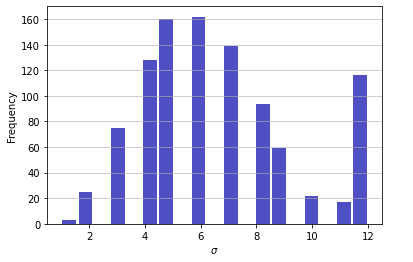
\includegraphics[height=8cm, width=8cm]{images/hamming_basic}
	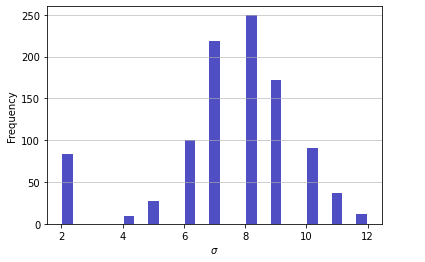
\includegraphics[height=8cm, width=8cm]{images/n_hamming}
	\caption{$ \sigma $ between the vectors and their recovered using the basic threshold iterative algorithm (left) and the normalized threshold iterative algorithm (right)for 3000 vectors}
\end{figure}
%It can be seen that the differences trend is almost the natural distribution. Where as these results are considered as desired but in the above example we relaxed the constraints. In the next section we focus on (BIHT) as our main target of tests.

Now lets test the probability of exact recovery of the algorithm. We ran a 100 simulation of a sample of 100 ($ n =100 $) and we took different values of $ m $ (tests) each time, that is we increase $ m $ be 5 up to $ n $.    

\begin{figure}[H]
	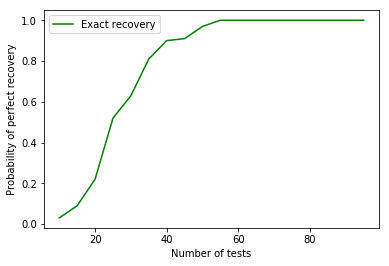
\includegraphics[height=8cm, width=8cm]{images/basic_exa}
	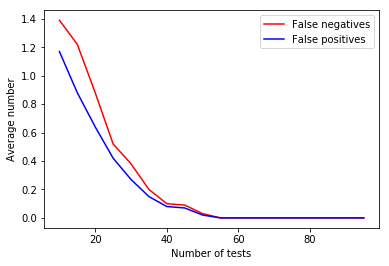
\includegraphics[height=8cm, width=8cm]{images/basic_false}
	\caption{This figure shows the probability of exact recovery (left) and  the average of false positive and false negatives vs the number of tests m (right), with number of individuals  = 100 and the number of defectives 2}
\end{figure}

\section{Binary iterative hard thresholding performance}

In this section we apply some tests on the binary iterative thresholding algorithm. We chose this algorithms as it is convenient to work with, because of its binary nature, as well as its robustness and stability which is shown in \cite{biht}. 

Primarily, we are testing the probability of exact recovery, specificity (false positive), and sensitivity (false negative). We will also include the $ \sigma $ test mentioned above. 

We run a number of simulations, in each of which we change the number of tests $ m $ according to the number individuals to be tested. 

The following graphs represent results from simulating the test 100 times with different number of individuals participating in the test.  

It is important that in both of following results the gradient descent (step size)  is kept fixed at $ \mu = 0.001 $

 \begin{figure}[H]
	%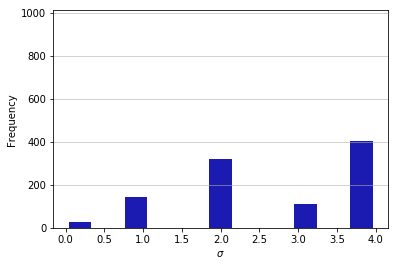
\includegraphics[height=8cm, width=8cm]{images/sigma_biht}
	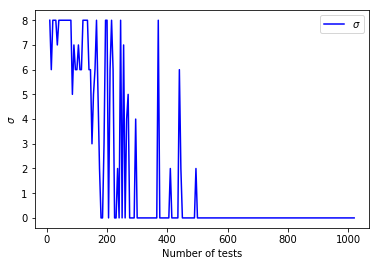
\includegraphics[height=8cm, width=8cm]{images/sigmavsm}
	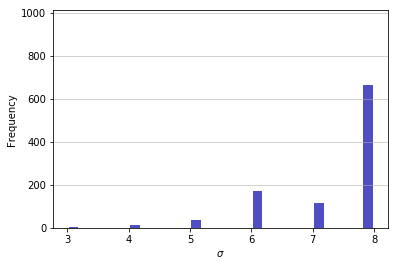
\includegraphics[height=8cm, width=8cm]{images/sigma_512}
	\caption{$ \sigma $ vs the number of tests $ m $ on the right and $ \sigma $ between the vectors and their recovered using the binary threshold iterative algorithm (BIHT) simulated 1000}
	\label{sigma}
\end{figure}
\begin{figure}[H]
	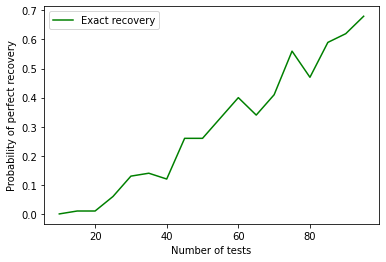
\includegraphics[height=8cm, width=8cm]{images/index1}
	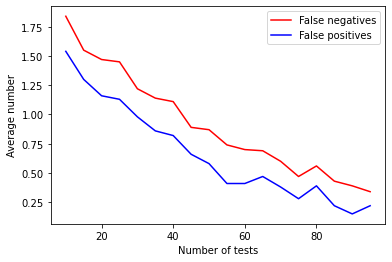
\includegraphics[height=8cm, width=8cm]{images/index}
	\caption{This figure shows the probability of exact recovery (left) and  the average of false positive and false negatives vs the number of tests m (right), with number of individuals  = 512 and the number of defectives 2, with $ \mu = 0.001 $}
	\label{exat}
\end{figure}

%\begin{figure}[H]
%	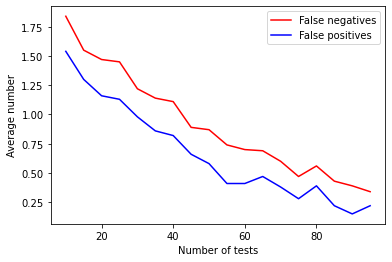
\includegraphics[height=9cm, width=8cm]{images/index}
%	\caption{This figure shows the average of false positive and false negatives vs the number of tests m, with number of individuals  = 100 and the number of defectives 2}
%\end{figure}

Next we increase the number of individuals and watch the three indicators mentioned above, taking the same test for 512, and 1024 individuals also keeping the number defectives low. 

\begin{figure}[H]
	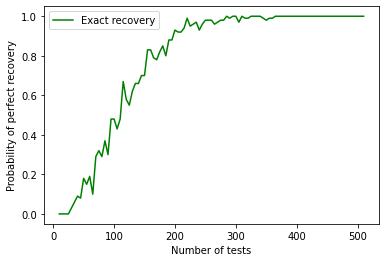
\includegraphics[height=8cm, width=8cm]{images/512ex}
	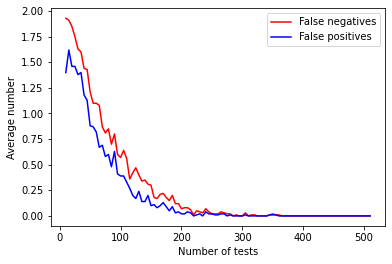
\includegraphics[height=8cm, width=8cm]{images/512fal}
	\caption{This figure shows the probability of exact recovery (left) and  the average of false positive and false negatives vs the number of tests m (right), with number of individuals  = 512 and the number of defectives 2, with $ \mu = 0.001 $}
	\label{exat1}
\end{figure}

Now we change the gradient descent $ \mu $, we set to $ 0.1 $ which relatively bigger than what chose first $ 0.001 $.

\begin{figure}[H]
	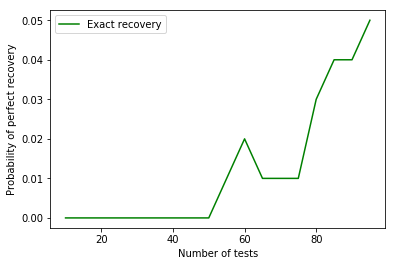
\includegraphics[height=8cm, width=8cm]{images/exa_mu}
	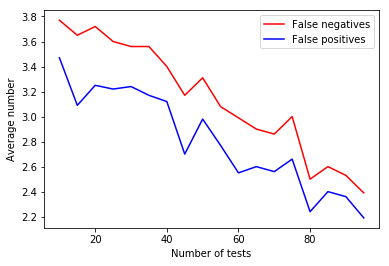
\includegraphics[height=8cm, width=8cm]{images/fal_mu}
	\caption{This figure shows the probability of exact recovery (left) and  the average of false positive and false negatives vs the number of tests m (right), with number of individuals  = 512 and the number of defectives 2, here $ \mu = 0.1 $}
	\label{mu}
\end{figure}


\subsection{Notes on the results of the BIHT simulation} 


\begin{itemize}
	\item The $ \sigma $ test that we run on the algorithm roughly tells us the convergence of the algorithm, where as we can see in  \ref{sigma} that with simulating the recovery 1000 times, most the $ \sigma $s are around $ 2d $, being the number of defectives. 
	
	\item The exact (perfect) recovery probability increases with increasing the number of tests $ m $,  but it noticed that from \ref{exat} on the left, \ref{exat1}, with the increase of $ n $, the algorithm starts to be more efficient, and it gives an exact recovery of probability of 1 earlier.    
	\item The false-positives and false-negative starts to fall sharply with increase of but with number of tests approaches certain point they being to stabilize at 0 \ref{exat1} on the right. 
	
	\item As $ \mu $ being very small the curves starts to be smother \ref{exat1} and \ref{mu}.    
\end{itemize}
 \section{Python code}
 
 The codes that are used in this thesis are available at: \href{https://github.com/KhalidOmer/School_thesis/tree/main}{github.com/KhalidOmer}
 
 
 The file README.md contains a brief description of the codes and what they do as well as how to
 run them. % through 3. model, to 4. analysis & results
%\chapter{The Second Squared Chapter}

An average dissertation may contain five chapters, but I didn't plan my work properly
and then ran out of time. I spent too much time positioning my figures and worrying
about my preferred typographic style, rather than just using what was provided.
I wasted days bolding section headings and using double slash line endings, and 
had to remove them all again. I spent sleepless nights configuring manually numbered lists
to use the \LaTeX\ environments because I didn't use them from the start or understand
how to search and replace easily with texmaker.

Everyone has to take some shortcuts
at some point to meet deadlines. Time did not allow to test model 
B as well. So I'll skip right ahead and put that under my Future Work section.


\section{This is a section} 
Text text text text text text text text text text text text text text
text text text text text text text text text text text text text text
text text text text text text text text text text text text text text
text text text text text text text text text text text text text text
text text text text text. 

Some dissertations may have 3, 4 or 5 chapters. This is just an example. 

Now you're demonstrating pure talent and newly acquired skills. 
Perhaps some persistence. Definitely some inspiration. What was that about perspiration? 
Some team work helps, so every now and then why not browse your friends' dissertations and provide
some constructive feedback?
 % You do not need to have exactly 4 chapters.
% Note LaTeX Produce an error when \\ is used in normal text 
\chapter*{Conclusion}
\addcontentsline{toc}{chapter}{Conclusion}

The idea of group testing is that we divide the population into groups. For each group then mix the samples drawn from each individual in the group and test the mixture. If the result of the test comes out negative then the group is free of the virus and if the result comes out positive then at least one individual of the group is infected. 


The goal of group testing research is to minimize the number of tests required to identify infected individuals in a population.  The problem is equivalent to solve a system of linear equations, with the number of equations being less the number of the unknowns.  Generally, there are two types of group testings, adaptive tests and non-adaptive test. In this work we consider the non-adaptive tests, where the tests are fixed in advance and conducted in parallel.


We present two topics here, first, the construction of efficient test designs. With the perfect design we can reduce the cost of detection, time and storage wise.  The second we review an algorithm that works on retrieving the missing information.  Here we verify that The Hard thresholding algorithms are robust and accurate in the decoding process.   % Conclusion is usually a chapter itself. 
% This is where we stop counting pages.
% Acknowledgements and References are not counted.
%----------------------------------------------------------------------------------------
\appendix
% Note LaTeX Produce an error when \\ is used in normal text 
\chapter{}
\section{Norm}

A norm of a vector space is a mapping that associates with each vector $ v $ a real number $||v||$ such that the following properties are satisfied for all vectors $ u, v $ and all scalars $ c \in \mathbb{R} $; 
\begin{enumerate}
	\item $ ||v|| \geq 0 $ and $ ||v|| = 0 $ if and only if $ v = 0 $.
	\item $||cv|| = |c| ||v||$.
	\item $||u+v|| \leq ||u|| + ||v||$
\end{enumerate}
The general norm in $ \mathbb{R} $ is defined as follows: 
\begin{equation}\label{key}
||v||_p = (|v_1|^p + ... + |v_n|^p)^{\frac{1}{p}}
\end{equation}
The first norm $ ||v||_1 $ also known as the taxicab is then obtained by setting $ p = 1 $ \begin{equation}\label{key}
||v||_1 = |v_1| + |v_2| + ... + |v_n|
\end{equation}
The second norm of the usual euclidean norm is obtained by setting $ p = 2 $ \begin{equation}\label{key}
||v||_2 = (|v_1|^2+...+|v_n|^2)^{\frac{1}{2}}
\end{equation} 

While as for the $ ||v||_0 $ or the pseudo norm is actually a comparison tool rather being the literal norm defined above, the $ ||v||_0 $ or $ l_0 $ as refereed to in the text  between counts the number of nonzero components in a vector. 
\subsection{Matrix norms induced by  p-norms}
A matrix norm on $ M_{nn} : V^{m\times n} \longrightarrow \mathbf{R}$ is a mapping that associates with $ m\times n $ matrix $ A $ a real number $ ||A|| $ called the norm of $ A $, such that the following properties are satisfied for all $ m \times n $ matrices and scalar $ \alpha \in V$ \begin{enumerate}
	\item $ ||A|| \geq 0 $.
	\item $ ||A|| = 0 \Longleftrightarrow A = 0_{m\times n} $. 
	\item $ ||\alpha A|| = |\alpha| ||A||$.
	\item $ ||A+B|| \leq ||A|| + ||B|| $.
\end{enumerate}

For $ 1 \geq p \leq \infty$ the corresponding operator norm is \begin{equation} ||A||_p = sup_{x \neq 0} \frac{||Ax||_p}{||x||_p} \end{equation} 
For the special cases $ p = 1,2$ the matrix norm is defined as follows: \begin{equation}
||A||_1 = max_{1\leq j \leq n} \sum_{i =1}^{m} |a_{ij} |
\end{equation}
\begin{equation}
||A||_2 = \sigma_{max} (A) 
\end{equation} where $\sigma_{max} (A)$ is the square root of the largest eigen value of $ AA^{T} $.

\section{Python code}

The codes that are used in this thesis are available at: \href{https://github.com/KhalidOmer/School_thesis/tree/main}{github.com/KhalidOmer}


The file README.md contains a brief description of the codes and what they do as well as how to
run them.




%----------------------------------------------------------------------------------------
% THE BIBLIOGRAPHY 
% Bibliography styles define how the bibliography is listed and formatted.
% This is part of the FMS house style and is only changed under exceptional
% circumstances
\renewcommand{\bibname}{References}
\nocite{*}
\addcontentsline{toc}{chapter}{References}
% 
% You should not repeat The label, For example "Ans07" should be used for only one ref. 
% Always separate AUTHORs by ", "
% AUTHOR1, AUTHOR2, AUTHOR3, AUTHOR4, ....., and AUTHORX
% where AUTHORX is   Lastname INITIAL of Firstname 
% Put ALL the authors, not et al. 
%
% Name of the Article/Book hould be Italic
%
% Article Volume should be Bold
%
% When you get arbitrary downloads ALWAYS check the copyright, and ask or inform
% the institution/author if this is required. Citing is not enough, some
% material may not be used. 
%
% For web published items, because they can change, put YEAR = "Accessed in April 2012",
% and if the item has a publish date, put that in the HOWPUBLISHED field after
% the institutions's name, (then publish date, then \url{}).
% Always find the original URL, not some Google Docs upload where you saved it
%
\begin{thebibliography}{199}
%%
% Article example
%%
%\bibitem{ref4} Vermolen F., Gefen A., \emph{Semi-stochastic cell-level computational modelling of cellular forces: application to contractures in burns and cyclic loading}. Biomech Model Mechanobiol, 2015: p. 1-15.
%%
%\bibitem{ref2} authors last name initial., \emph{Name of the article}. Journal, year. {\bf{volume}}(issue): pages.
%%
% Book example
%\bibitem{Bah99} Bahra A., Cikurel K., \emph{Neurology}, Elsevier Health Sciences, 1999.
%%
%\bibitem{ref3} author last name initial., \emph{ name of the book}, publisher, year.
%%
\bibitem{mathbook}{
		title={An invitation to compressive sensing},
		author={Foucart, Simon and Rauhut, Holger},
		booktitle={A mathematical introduction to compressive sensing},
		pages={1--39},
		year={2013},
		publisher={Springer}
	}
\bibitem{kubook}{
	title={Combinatorial group testing and its applications},
	author={Du, Dingzhu and Hwang, Frank K and Hwang, Frank},
	volume={12},
	year={2000},
	publisher={World Scientific}
}

\bibitem{aldridge}{
	title={Group testing: an information theory perspective},
	author={Aldridge, Matthew and Johnson, Oliver and Scarlett, Jonathan and others},
	journal={Foundations and Trends{\textregistered} in Communications and Information Theory},
	volume={15},
	number={3-4},
	pages={196--392},
	year={2019},
	publisher={Now Publishers, Inc.}
}
\bibitem{ref3}{
	title={Hard thresholding pursuit: an algorithm for compressive sensing},
	author={Foucart, Simon},
	journal={SIAM Journal on numerical analysis},
	volume={49},
	number={6},
	pages={2543--2563},
	year={2011},
	publisher={SIAM}
}
\bibitem{bluemensath}{
	title={Iterative thresholding for sparse approximations},
	author={Blumensath, Thomas and Davies, Mike E},
	journal={Journal of Fourier analysis and Applications},
	volume={14},
	number={5},
	pages={629--654},
	year={2008},
	publisher={Springer}
}
\bibitem{bluementh}{
	title={Iterative hard thresholding: Theory and practice},
	author={Blumensath, Thomas},
	journal={Inst. Digit. Commun., Signal Image Process., Univ. Edinburgh, Edinburgh, UK, Tech. Rep},
	year={2009}
}
\bibitem{mutal}{
	title = {Optimized projections for compressed sensing via direct mutual coherence minimization},
	journal = {Signal Processing},
	volume = {151},
	pages = {45-55},
	year = {2018},
	issn = {0165-1684},
	doi = {https://doi.org/10.1016/j.sigpro.2018.04.020},
	url = {https://www.sciencedirect.com/science/article/pii/S0165168418301464},
	author = {Canyi Lu and Huan Li and Zhouchen Lin}}
\bibitem{ripg}{
	title={A simple proof of the restricted isometry property for random matrices},
	author={Baraniuk, Richard and Davenport, Mark and DeVore, Ronald and Wakin, Michael},
	journal={Constructive Approximation},
	volume={28},
	number={3},
	pages={253--263},
	year={2008},
	publisher={Springer}
}
\bibitem{IEEE}{
	title={Improved algorithms for non-adaptive group testing with consecutive positives},
	author={Bui, Thach V and Cheraghchi, Mahdi and Nguyen, Thuc D},
	booktitle={2021 IEEE International Symposium on Information Theory (ISIT)},
	pages={1961--1966},
	year={2021},
	organization={IEEE}
}
\bibitem{RIP}{
	title = {The restricted isometry property and its implications for compressed sensing},
	journal = {Comptes Rendus Mathematique},
	volume = {346},
	number = {9},
	pages = {589-592},
	year = {2008},
	issn = {1631-073X},
	doi = {https://doi.org/10.1016/j.crma.2008.03.014},
	url = {https://www.sciencedirect.com/science/article/pii/S1631073X08000964},
	author = {Emmanuel J. Candès}}
\bibitem{radar}{
	title = {Academic press library in signal processing, Volume 7: Array, radar and communications engineering},
	author = {Chellappa, Rama and Theodoridis, S.},
	year = {2017},
	month = {12},
	pages = {1-626},
	journal = {Academic Press Library in Signal Processing, Volume 7: Array, Radar and Communications Engineering},
	doi = {10.1016/C2016-0-00738-6}
}
\bibitem{analysis}{
	title="Sparse Recovery Algorithms: Sufficient Conditions in Terms of RestrictedIsometry Constants",
	author="Foucart, Simon",
	editor="Neamtu, Marian
	and Schumaker, Larry",
	booktitle="Approximation Theory XIII: San Antonio 2010",
	year="2012",
	publisher="Springer New York",
	address="New York, NY",
	pages="65--77",}
\bibitem{binary}{
	title={1-bit compressive sensing},
	author={Boufounos, Petros T and Baraniuk, Richard G},
	booktitle={2008 42nd Annual Conference on Information Sciences and Systems},
	pages={16--21},
	year={2008},
	organization={IEEE}
}


\bibitem{biht}{
	author    = {Laurent Jacques and
		Jason N. Laska and
		Petros Boufounos and
		Richard G. Baraniuk},
	title     = {Robust 1-Bit Compressive Sensing via Binary Stable Embeddings of Sparse
		Vectors},
	journal   = {CoRR},
	volume    = {abs/1104.3160},
	year      = {2011},
	url       = {http://arxiv.org/abs/1104.3160},
	eprinttype = {arXiv},
	eprint    = {1104.3160},
	timestamp = {Mon, 13 Aug 2018 16:46:15 +0200},
	biburl    = {https://dblp.org/rec/journals/corr/abs-1104-3160.bib},
	bibsource = {dblp computer science bibliography, https://dblp.org}
}




\end{thebibliography} 
%\bibliographystyle{apa}
%\bibliography{references}
\end{document}
%---------------------------------------------------------------------------------------
